\documentclass[12pt,a4paper]{article}
\usepackage[utf8]{inputenc}
\usepackage[margin=1in]{geometry}
\usepackage{graphicx}
\usepackage{booktabs}
\usepackage{longtable}
\usepackage{array}
\usepackage{multirow}
\usepackage{float}
\usepackage{caption}
\usepackage{subcaption}
\usepackage{amsmath}
\usepackage{hyperref}
\usepackage{fancyhdr}
\usepackage{titlesec}
\usepackage{xcolor}
\usepackage{pgfplots}
\pgfplotsset{compat=1.18}

% Page style
\pagestyle{fancy}
\fancyhf{}
\rhead{Assignment 3}
\lhead{Project Management}
\rfoot{Page \thepage}

\begin{document}

% Custom Cover Page
\begin{titlepage}
\centering
\vspace*{1cm}

{\LARGE \textbf{FAST National University of Computer and Emerging Sciences}}\\[0.5cm]
{\large Islamabad Campus}\\[2cm]

{\huge \textbf{Assignment 3}}\\[0.5cm]
{\Large Project Scheduling, Network Analysis,}\\
{\Large and Cost Management}\\[1.5cm]

{\large \textbf{Course:} Project Management}\\[0.3cm]
{\large \textbf{Project:} Mindful Eating Agent}\\[2cm]

\begin{flushleft}
\large
\textbf{Submitted By:}\\[0.5cm]
\begin{tabular}{ll}
\textbf{Name} & \textbf{Roll Number}\\
\hline
Dawood Hussain & 22i-2410\\
Gulsher Khan & 22i-2637\\
Ahsan Faraz & 22i-8791\\
\end{tabular}\\[0.5cm]
\textbf{Section:} E\\[2cm]
\end{flushleft}

\vfill

{\large \textbf{Submission Date:} November 3, 2025}

\end{titlepage}

\thispagestyle{empty}

\newpage
\tableofcontents
\newpage

\section{Introduction}
This document presents the third deliverable for the Mindful Eating Agent project, focusing on timeline estimation, network diagram analysis, and comprehensive cost estimation with earned value management. The project aims to develop an AI-powered mobile application that helps users track their nutritional intake through image recognition and provides personalized dietary recommendations.


\section{Task 1: Timeline Estimation and Scheduling of WBS Items}

\subsection{Overview}
Based on the Work Breakdown Structure developed in Assignment 2, we have estimated timelines, durations, dependencies, and assigned responsible team members for all project activities. The project spans 112 days from September 1, 2025, to December 15, 2025.

\subsection{Work Breakdown Structure with Timeline}

The following figures present the detailed Work Breakdown Structure with complete timeline information, including task durations, start/finish dates, dependencies, and team member assignments.

\begin{figure}[H]
\centering
\includegraphics[width=\textwidth,height=0.85\textheight,keepaspectratio]{wbs_img_1.png}
\caption{Work Breakdown Structure - Part 1: Project phases and major deliverables}
\label{fig:wbs1}
\end{figure}

\begin{figure}[H]
\centering
\includegraphics[width=\textwidth,height=0.85\textheight,keepaspectratio]{wbs_img_2.png}
\caption{Work Breakdown Structure - Part 2: Detailed task breakdown with scheduling information}
\label{fig:wbs2}
\end{figure}

\textbf{Interactive WBS Breakdown:} For a detailed interactive view of the complete Work Breakdown Structure with all task details, dependencies, and scheduling information, please visit: 

\url{https://www.notion.so/28c7b62d9611802fb54ed11d61414829?v=28c7b62d9611818e8763000c4dd51ba6}


\subsection{Justification for Major Work Package Durations}

\subsubsection{AI/ML Module Development (24 days)}
This is the most critical and time-intensive component of the project. The duration is justified by:
\begin{itemize}
    \item \textbf{Model Training (9 days):} Training a TensorFlow CNN model on 100,000+ food images requires multiple iterative training cycles and hyperparameter tuning to achieve the required 95\% accuracy threshold.
    \item \textbf{Model Validation (3 days):} Comprehensive testing on diverse datasets to measure accuracy, precision, and recall, including identification of edge cases.
    \item \textbf{Model Optimization (2 days):} Model compression and inference time optimization to meet the <2 second response requirement for mobile deployment.
    \item \textbf{Model Integration (2 days):} Integration with backend API, implementing inference endpoints, and robust error handling.
\end{itemize}

\subsubsection{Mobile App Development (28 days)}
The longest single task in the project, justified by:
\begin{itemize}
    \item Cross-platform development using React Native for both iOS and Android
    \item Complex camera integration for real-time food image capture
    \item Implementation of offline capability for food logging
    \item Comprehensive UI/UX implementation across multiple screens
    \item Integration with backend APIs and AI model endpoints
\end{itemize}


\subsubsection{Backend API Development (14 days)}
Justified by the need to develop multiple RESTful endpoints including:
\begin{itemize}
    \item User authentication and authorization system
    \item Food logging and retrieval APIs
    \item Recommendation engine integration
    \item Database operations and query optimization
    \item API documentation and testing
\end{itemize}

\subsubsection{Requirements Gathering (6 days)}
Comprehensive requirements collection through:
\begin{itemize}
    \item Interviews and surveys with 50+ stakeholders
    \item Multiple workshops to gather functional and non-functional requirements
    \item Documentation and validation of requirements
    \item Stakeholder review and approval cycles
\end{itemize}

\subsubsection{Integration Testing (10 days)}
Critical phase requiring:
\begin{itemize}
    \item End-to-end testing of mobile app with backend and AI model
    \item Performance testing under various load conditions
    \item Bug identification and resolution
    \item Regression testing after fixes
    \item Final validation before deployment
\end{itemize}


\subsubsection{Continuous Activities}
Four activities span the entire or significant portions of the project:
\begin{itemize}
    \item \textbf{Project Coordination (106 days):} Continuous oversight required throughout the project lifecycle to ensure team coordination and timely delivery.
    \item \textbf{Risk Management (106 days):} Ongoing monitoring to identify, assess, and mitigate risks as they emerge.
    \item \textbf{Quality Management (106 days):} Quality assurance needed throughout all phases to ensure deliverables meet acceptance criteria.
    \item \textbf{Change Management (76 days):} Active from project authorization through development completion to handle scope changes and ensure proper change control.
\end{itemize}

\subsection{Team Member Responsibilities}
\begin{itemize}
    \item \textbf{Dawood Hussain (Project Manager):} Project coordination, stakeholder management, requirements gathering, risk planning, UAT coordination, and project closure activities.
    \item \textbf{Gulsher Khan (Technical Lead):} System architecture design, backend API development, mobile app development, environment setup, and deployment activities.
    \item \textbf{Ahsan Faraz (AI/ML Developer):} AI/ML module development including model training, validation, optimization, database design, and functional testing.
\end{itemize}


\newpage
\section{Task 2: Network Diagram (AON) and Slack Analysis}

\subsection{Activity-on-Node (AON) Network Diagram}

The network diagram below illustrates the logical sequence and dependencies among all project activities using Activity-on-Node notation. Tasks are represented as nodes, and dependencies are shown as arrows. The critical path is highlighted in red with solid lines, while non-critical activities are shown in blue with dashed lines.

\begin{figure}[H]
\centering
\includegraphics[width=\textwidth,height=0.9\textheight,keepaspectratio]{network_diagram_image.png}
\caption{Activity-on-Node Network Diagram showing project activities, dependencies, and critical path}
\label{fig:network}
\end{figure}


\subsection{Critical Path Analysis}

The critical path represents the longest sequence of dependent activities that determines the minimum project duration. For the Mindful Eating Agent project:

\begin{itemize}
    \item \textbf{Total Project Duration:} 112 days
    \item \textbf{Critical Path Activities:} 32 activities with Total Slack = 0
    \item \textbf{Non-Critical Activities:} 8 activities with Total Slack > 0
\end{itemize}

\textbf{Critical Path Sequence:}
\begin{enumerate}
    \item Market Research (1.2.1) $\rightarrow$ Stakeholder Identification (1.2.2)
    \item Business Case Development (1.2.4) $\rightarrow$ Project Authorization (M1)
    \item Requirements Gathering (1.3.1) $\rightarrow$ Requirements Approved (M2)
    \item System Architecture Design (1.3.2) $\rightarrow$ Risk Planning (1.3.6)
    \item Design Approved (M3) $\rightarrow$ Environment Setup (1.4.1)
    \item Backend API Development (1.4.2) $\rightarrow$ Mobile App Development (1.4.4)
    \item Integration Testing (1.4.5) $\rightarrow$ Development Complete (M4)
    \item Functional Testing (1.5.1) $\rightarrow$ Production Deployment (1.5.4)
    \item Go Live (M5) $\rightarrow$ Project Closure activities (1.6.1-1.6.4)
\end{enumerate}


\subsection{Slack Analysis}

\subsubsection{Total Slack and Free Slack Calculations}

Table \ref{tab:slack} presents the Total Slack (TS) and Free Slack (FS) for all project activities. Total Slack represents the amount of time an activity can be delayed without delaying the project completion, while Free Slack indicates the delay possible without affecting successor activities.

\tiny
\begin{longtable}{|>{\centering\arraybackslash}p{0.8cm}|>{\raggedright\arraybackslash}p{2.8cm}|>{\centering\arraybackslash}p{0.6cm}|>{\centering\arraybackslash}p{0.5cm}|>{\centering\arraybackslash}p{0.5cm}|>{\centering\arraybackslash}p{0.5cm}|>{\centering\arraybackslash}p{0.5cm}|>{\centering\arraybackslash}p{0.6cm}|>{\centering\arraybackslash}p{0.6cm}|>{\centering\arraybackslash}p{0.5cm}|>{\raggedright\arraybackslash}p{1.2cm}|>{\raggedright\arraybackslash}p{1.5cm}|>{\centering\arraybackslash}p{0.8cm}|}
\caption{Slack Analysis for All Project Activities} \label{tab:slack} \\
\hline
\textbf{WBS ID} & \textbf{Task Name} & \textbf{Dur} & \textbf{ES} & \textbf{EF} & \textbf{LS} & \textbf{LF} & \textbf{Total Slack} & \textbf{Free Slack} & \textbf{CP} & \textbf{Predecessors} & \textbf{Phase} & \textbf{Risk} \\
\hline
\endfirsthead

\multicolumn{13}{c}%
{{\tablename\ \thetable{} -- continued from previous page}} \\
\hline
\textbf{WBS ID} & \textbf{Task Name} & \textbf{Dur} & \textbf{ES} & \textbf{EF} & \textbf{LS} & \textbf{LF} & \textbf{Total Slack} & \textbf{Free Slack} & \textbf{CP} & \textbf{Predecessors} & \textbf{Phase} & \textbf{Risk} \\
\hline
\endhead

\hline \multicolumn{13}{|r|}{{Continued on next page}} \\ \hline
\endfoot

\hline
\endlastfoot

1.1.1 & Project Coordination & 106 & 0 & 106 & 0 & 106 & 0 & 0 & Yes & None & Continuous & HIGH \\
1.1.2 & Risk Management & 106 & 0 & 106 & 0 & 106 & 0 & 0 & Yes & None & Continuous & HIGH \\
1.1.3 & Change Management & 76 & 14 & 90 & 14 & 90 & 0 & 0 & Yes & 1.1.1 & Continuous & HIGH \\
1.1.4 & Quality Management & 106 & 0 & 106 & 0 & 106 & 0 & 0 & Yes & None & Continuous & HIGH \\
1.2.1 & Market Research & 5 & 0 & 5 & 0 & 5 & 0 & 0 & Yes & None & Phase 1 & HIGH \\
1.2.2 & Stakeholder ID & 5 & 5 & 10 & 5 & 10 & 0 & 0 & Yes & None & Phase 1 & HIGH \\
1.2.3 & Feasibility Study & 7 & 5 & 12 & 8 & 15 & \textbf{3} & 0 & No & None & Phase 1 & MED \\
1.2.4 & Business Case Dev & 5 & 10 & 15 & 10 & 15 & 0 & 0 & Yes & 1.2.2, 1.2.3 & Phase 1 & HIGH \\
M1 & Project Authorization & 0 & 15 & 15 & 15 & 15 & 0 & 0 & Yes & 1.2.4 & Phase 1 & HIGH \\
1.3.1 & Requirements Gathering & 6 & 15 & 21 & 15 & 21 & 0 & 0 & Yes & M1 & Phase 2 & HIGH \\
M2 & Requirements Approved & 0 & 21 & 21 & 21 & 21 & 0 & 0 & Yes & 1.3.1 & Phase 2 & HIGH \\
1.3.2 & System Architecture & 8 & 21 & 29 & 21 & 29 & 0 & 0 & Yes & 1.3.1 & Phase 2 & HIGH \\
1.3.3 & UI/UX Design & 11 & 21 & 32 & 29 & 40 & \textbf{8} & \textbf{8} & No & 1.3.1 & Phase 2 & LOW \\
1.3.4 & Database Design & 10 & 24 & 34 & 30 & 40 & \textbf{6} & \textbf{6} & No & 1.3.1 & Phase 2 & MED \\
1.3.5 & Schedule Development & 8 & 29 & 37 & 32 & 40 & \textbf{3} & \textbf{3} & No & 1.3.2 & Phase 2 & MED \\
1.3.6 & Risk Planning & 7 & 33 & 40 & 33 & 40 & 0 & 0 & Yes & 1.3.5 & Phase 2 & HIGH \\
M3 & Design Approved & 0 & 40 & 40 & 40 & 40 & 0 & 0 & Yes & 1.3.6 & Phase 2 & HIGH \\
1.4.1 & Environment Setup & 10 & 40 & 50 & 40 & 50 & 0 & 0 & Yes & M3 & Phase 3 & HIGH \\
1.4.2 & Backend API Dev & 14 & 44 & 58 & 44 & 58 & 0 & 0 & Yes & 1.4.1 & Phase 3 & CRIT \\
1.4.3 & AI/ML Module Dev & 24 & 44 & 68 & 44 & 68 & 0 & 0 & Yes & 1.3.4 & Phase 3 & CRIT \\
1.4.3.1 & Model Training & 9 & 44 & 53 & 44 & 53 & 0 & 0 & Yes & 1.4.3 & Phase 3 & CRIT \\
1.4.3.2 & Model Validation & 3 & 53 & 56 & 53 & 56 & 0 & 0 & Yes & 1.4.3.1 & Phase 3 & CRIT \\
1.4.3.3 & Model Optimization & 2 & 56 & 58 & 56 & 58 & 0 & 0 & Yes & 1.4.3.2 & Phase 3 & CRIT \\
1.4.3.4 & Model Integration & 2 & 58 & 60 & 58 & 60 & 0 & 0 & Yes & 1.4.3.3 & Phase 3 & CRIT \\
1.4.4 & Mobile App Dev & 28 & 58 & 86 & 58 & 86 & 0 & 0 & Yes & 1.4.2 & Phase 3 & CRIT \\
1.4.5 & Integration Testing & 10 & 86 & 96 & 86 & 96 & 0 & 0 & Yes & 1.4.4, 1.4.3.4 & Phase 3 & CRIT \\
M4 & Development Complete & 0 & 96 & 96 & 96 & 96 & 0 & 0 & Yes & 1.4.5 & Phase 3 & CRIT \\
1.5.1 & Functional Testing & 6 & 96 & 102 & 96 & 102 & 0 & 0 & Yes & M4 & Phase 4 & HIGH \\
1.5.2 & User Acceptance Test & 5 & 100 & 105 & 101 & 106 & \textbf{1} & \textbf{1} & No & 1.5.1 & Phase 4 & MED \\
1.5.3 & Prod Env Setup & 4 & 96 & 100 & 102 & 106 & \textbf{6} & \textbf{6} & No & 1.4.5 & Phase 4 & LOW \\
1.5.4 & Production Deploy & 2 & 105 & 107 & 105 & 107 & 0 & 0 & Yes & 1.5.3, 1.5.2 & Phase 4 & HIGH \\
1.5.5 & User Training & 2 & 105 & 107 & 105 & 107 & 0 & 0 & Yes & 1.5.2 & Phase 4 & HIGH \\
M5 & Go Live & 0 & 107 & 107 & 107 & 107 & 0 & 0 & Yes & 1.5.4 & Phase 4 & HIGH \\
1.6.1 & Deliverable Accept & 2 & 107 & 109 & 107 & 109 & 0 & 0 & Yes & M5 & Phase 5 & HIGH \\
1.6.2 & Knowledge Transfer & 1 & 109 & 110 & 109 & 110 & 0 & 0 & Yes & 1.6.1 & Phase 5 & HIGH \\
1.6.3 & Lessons Learned & 1 & 110 & 111 & 110 & 111 & 0 & 0 & Yes & 1.6.2 & Phase 5 & HIGH \\
1.6.4 & Admin Closure & 1 & 111 & 112 & 111 & 112 & 0 & 0 & Yes & 1.6.3 & Phase 5 & HIGH \\
M6 & Project Closed & 0 & 112 & 112 & 112 & 112 & 0 & 0 & Yes & 1.6.4 & Phase 5 & HIGH \\
\hline
\multicolumn{13}{|l|}{\textit{Note: Dur=Duration (days), ES=Early Start, EF=Early Finish, LS=Late Start, LF=Late Finish, CP=Critical Path, MED=Medium, CRIT=Critical}} \\
\end{longtable}
\normalsize


\subsubsection{Parallel Paths Analysis}

The project contains several parallel paths that allow concurrent execution of activities:

\textbf{Parallel Path 1 - Planning Phase (Days 21-40):}
\begin{itemize}
    \item \textbf{Critical:} System Architecture Design (8 days) $\rightarrow$ Risk Planning (7 days)
    \item \textbf{Non-Critical:} UI/UX Design (11 days, TS=8 days)
    \item \textbf{Non-Critical:} Database Design (10 days, TS=6 days)
    \item \textbf{Non-Critical:} Schedule Development (8 days, TS=3 days)
\end{itemize}

These activities can be executed in parallel after Requirements Approval, with the critical path running through System Architecture and Risk Planning.

\textbf{Parallel Path 2 - Development Phase (Days 40-96):}
\begin{itemize}
    \item \textbf{Path A (Critical):} Environment Setup $\rightarrow$ Backend API $\rightarrow$ Mobile App Dev $\rightarrow$ Integration Testing
    \item \textbf{Path B (Critical):} AI/ML Module Development (runs parallel to Backend/Mobile) $\rightarrow$ Integration Testing
\end{itemize}

Both paths converge at Integration Testing (Day 86), making it a critical merge point.


\textbf{Parallel Path 3 - Testing \& Deployment Phase (Days 96-107):}
\begin{itemize}
    \item \textbf{Critical:} Functional Testing $\rightarrow$ Production Deployment
    \item \textbf{Non-Critical:} User Acceptance Testing (TS=1 day)
    \item \textbf{Non-Critical:} Production Environment Setup (TS=6 days)
    \item \textbf{Critical:} User Training (parallel to deployment)
\end{itemize}

\subsubsection{Activities with Highest Slack}

The following activities have the most scheduling flexibility:

\begin{enumerate}
    \item \textbf{UI/UX Design (TS=8 days, FS=8 days):} Can be delayed up to 8 days without impacting the project. This provides flexibility for design iterations and stakeholder feedback.
    
    \item \textbf{Production Environment Setup (TS=6 days, FS=6 days):} Has significant slack, allowing time for security approvals and infrastructure configuration without pressure.
    
    \item \textbf{Database Design (TS=6 days, FS=6 days):} Can accommodate additional time for schema optimization and scalability planning.
    
    \item \textbf{Feasibility Study (TS=3 days):} Provides some buffer for comprehensive technical and economic analysis.
    
    \item \textbf{Schedule Development (TS=3 days):} Allows time for detailed planning and resource allocation refinement.
\end{enumerate}


\newpage
\section{Task 3: Cost Estimation, Budgeting, and Earned Value Analysis}

\subsection{Cost Estimation and Budget at Completion (BAC)}

A comprehensive cost estimation has been prepared in Microsoft Excel, covering all project activities including labor, infrastructure, software licenses, and contingency reserves. The detailed breakdown is provided in the attached Excel file \texttt{wbs\_detailed\_breakdown.xlsx}.

\subsubsection{Cost Categories}

The project budget includes the following major cost categories:

\begin{table}[H]
\centering
\caption{Project Budget Summary}
\label{tab:budget}
\begin{tabular}{|l|r|r|}
\hline
\textbf{Cost Category} & \textbf{Amount (USD)} & \textbf{Percentage} \\
\hline
\textbf{Labor Costs} & & \\
\quad Project Manager (Dawood) & \$42,000 & 28.0\% \\
\quad Technical Lead (Gulsher) & \$48,000 & 32.0\% \\
\quad AI/ML Developer (Ahsan) & \$45,000 & 30.0\% \\
\hline
\textbf{Subtotal - Labor} & \$135,000 & 90.0\% \\
\hline
\textbf{Infrastructure \& Tools} & & \\
\quad AWS Cloud Services & \$4,500 & 3.0\% \\
\quad Development Tools \& Licenses & \$2,000 & 1.3\% \\
\quad Testing Infrastructure & \$1,500 & 1.0\% \\
\hline
\textbf{Subtotal - Infrastructure} & \$8,000 & 5.3\% \\
\hline
\textbf{Other Costs} & & \\
\quad Training \& Documentation & \$2,000 & 1.3\% \\
\quad Miscellaneous & \$1,000 & 0.7\% \\
\hline
\textbf{Subtotal - Other} & \$3,000 & 2.0\% \\
\hline
\textbf{Subtotal (Before Contingency)} & \$146,000 & 97.3\% \\
\hline
\textbf{Contingency Reserve (10\%)} & \$4,000 & 2.7\% \\
\hline
\textbf{Budget at Completion (BAC)} & \textbf{\$150,000} & \textbf{100.0\%} \\
\hline
\end{tabular}
\end{table}

\subsubsection{Detailed Cost Estimation Breakdown}

The following figures present the comprehensive cost estimation and budgeting spreadsheet with itemized costs, phase-wise breakdown, and budget summary.

\begin{figure}[H]
\centering
\includegraphics[width=\textwidth,keepaspectratio]{costEst-1.png}
\caption{Cost Estimation - Phase-wise breakdown (Part 1)}
\label{fig:cost1}
\end{figure}

\begin{figure}[H]
\centering
\includegraphics[width=\textwidth,keepaspectratio]{costEst-2.png}
\caption{Cost Estimation - Phase-wise breakdown (Part 2)}
\label{fig:cost2}
\end{figure}

\begin{figure}[H]
\centering
\includegraphics[width=\textwidth,keepaspectratio]{costEst-3.png}
\caption{Cost Estimation - Budget summary and contingency reserves}
\label{fig:cost3}
\end{figure}

\subsubsection{Cost Estimation Methodology}

\textbf{Labor Costs:}
\begin{itemize}
    \item \textbf{Project Manager:} \$375/day × 112 days = \$42,000
    \item \textbf{Technical Lead:} \$400/day × 120 days (includes overtime) = \$48,000
    \item \textbf{AI/ML Developer:} \$375/day × 120 days (includes overtime) = \$45,000
\end{itemize}

\textbf{Infrastructure Costs:}
\begin{itemize}
    \item AWS EC2, S3, RDS services for 4 months (dev + prod): \$4,500
    \item Development tools (IDEs, version control, CI/CD): \$2,000
    \item Testing infrastructure and tools: \$1,500
\end{itemize}

\textbf{Contingency Reserve:}
A 10\% contingency reserve (\$4,000) has been allocated to cover unforeseen risks such as:
\begin{itemize}
    \item Scope changes or requirement modifications
    \item Technical challenges in AI model development
    \item Extended testing or bug fixing requirements
    \item Infrastructure scaling needs
\end{itemize}

\textbf{Total Budget at Completion (BAC): \$150,000}


\subsection{Earned Value Management (EVM) Analysis}

\subsubsection{Project Status After 3 Months}

Assuming the project started on September 1, 2025, after three months (approximately 90 days), we are at December 1, 2025. Based on the project schedule:

\textbf{Planned Progress (as of Day 90):}
\begin{itemize}
    \item All planning phases completed (Initiation and Planning)
    \item Development phase in progress
    \item AI/ML Module Development should be near completion
    \item Mobile App Development should be in progress
    \item Integration Testing should be starting soon
\end{itemize}

\subsubsection{Assumptions for EVM Calculations}

\textbf{Planned Value (PV):}
Based on the project schedule, by Day 90, the following work should be completed:
\begin{itemize}
    \item All initiation activities (Days 0-15): 10\% of BAC = \$15,000
    \item All planning activities (Days 15-40): 15\% of BAC = \$22,500
    \item Development activities (Days 40-90): 50\% of development = 35\% of BAC = \$52,500
\end{itemize}
\textbf{PV = \$90,000} (60\% of project planned to be complete)


\textbf{Earned Value (EV):}
Actual work completed by Day 90:
\begin{itemize}
    \item Initiation phase: 100\% complete = \$15,000
    \item Planning phase: 100\% complete = \$22,500
    \item Development phase: 55\% complete (ahead of schedule) = 38.5\% of BAC = \$57,750
\end{itemize}
\textbf{EV = \$95,250} (63.5\% of project actually complete)

\textbf{Actual Cost (AC):}
Actual expenditure by Day 90:
\begin{itemize}
    \item Labor costs for 3 months: \$85,000
    \item Infrastructure and tools: \$6,500
    \item Other costs: \$2,000
\end{itemize}
\textbf{AC = \$93,500} (62.3\% of budget spent)

\subsubsection{Variance Analysis}

\textbf{(a) Cost Variance (CV) and Schedule Variance (SV):}

\begin{align*}
\text{Cost Variance (CV)} &= \text{EV} - \text{AC} \\
&= \$95,250 - \$93,500 \\
&= \textbf{+\$1,750}
\end{align*}

\begin{align*}
\text{Schedule Variance (SV)} &= \text{EV} - \text{PV} \\
&= \$95,250 - \$90,000 \\
&= \textbf{+\$5,250}
\end{align*}


\textbf{(b) Cost Performance Index (CPI) and Schedule Performance Index (SPI):}

\begin{align*}
\text{Cost Performance Index (CPI)} &= \frac{\text{EV}}{\text{AC}} \\
&= \frac{\$95,250}{\$93,500} \\
&= \textbf{1.019}
\end{align*}

\begin{align*}
\text{Schedule Performance Index (SPI)} &= \frac{\text{EV}}{\text{PV}} \\
&= \frac{\$95,250}{\$90,000} \\
&= \textbf{1.058}
\end{align*}

\textbf{(c) Interpretation of Results:}

\textbf{Schedule Performance:}
\begin{itemize}
    \item SV = +\$5,250 (positive) indicates the project is \textbf{ahead of schedule}
    \item SPI = 1.058 (>1.0) confirms the project is progressing 5.8\% faster than planned
    \item The team has completed 63.5\% of work when only 60\% was planned
    \item This is primarily due to efficient execution of the AI/ML module development
\end{itemize}

\textbf{Cost Performance:}
\begin{itemize}
    \item CV = +\$1,750 (positive) indicates the project is \textbf{under budget}
    \item CPI = 1.019 (>1.0) shows the project is getting \$1.019 worth of work for every \$1.00 spent
    \item The project is performing 1.9\% better than budgeted
    \item Cost efficiency is maintained despite being ahead of schedule
\end{itemize}

\textbf{Overall Assessment:}
The project is in excellent health, performing better than planned in both schedule and cost dimensions. The positive variances indicate effective project management and efficient resource utilization.


\textbf{(d) Estimate at Completion (EAC) using CPI:}

\begin{align*}
\text{Estimate at Completion (EAC)} &= \frac{\text{BAC}}{\text{CPI}} \\
&= \frac{\$150,000}{1.019} \\
&= \textbf{\$147,203}
\end{align*}

\textbf{Interpretation:}
The EAC of \$147,203 is \$2,797 less than the original BAC of \$150,000. This indicates:
\begin{itemize}
    \item The project is expected to finish \textbf{under budget} by approximately \$2,800
    \item Current cost performance trends suggest continued efficiency
    \item The project is performing \textbf{better than planned} from a cost perspective
    \item The contingency reserve may not be fully utilized
    \item This provides a buffer for any unforeseen issues in the remaining project phases
\end{itemize}

\textbf{(e) Schedule Estimate using SPI:}

\begin{align*}
\text{Estimated Duration} &= \frac{\text{Planned Duration}}{\text{SPI}} \\
&= \frac{112 \text{ days}}{1.058} \\
&= \textbf{105.9 days} \approx \textbf{106 days}
\end{align*}

Converting to months: $\frac{106 \text{ days}}{30 \text{ days/month}} = \textbf{3.53 months}$

\textbf{Interpretation:}
\begin{itemize}
    \item The project is expected to complete in approximately \textbf{3.5 months} instead of the planned 3.7 months (112 days)
    \item This represents a time savings of approximately \textbf{6 days}
    \item The project could potentially finish by \textbf{December 9, 2025} instead of December 15, 2025
    \item Early completion provides opportunities for extended testing or early deployment
    \item The schedule buffer can be used to accommodate any delays in critical path activities
\end{itemize}


\subsection{Earned Value Chart}

\textbf{(f) Earned Value Chart:}

Figure \ref{fig:ev_chart} presents the Earned Value chart showing the relationship between Planned Value (PV), Earned Value (EV), and Actual Cost (AC) over the project timeline.

\begin{figure}[H]
\centering
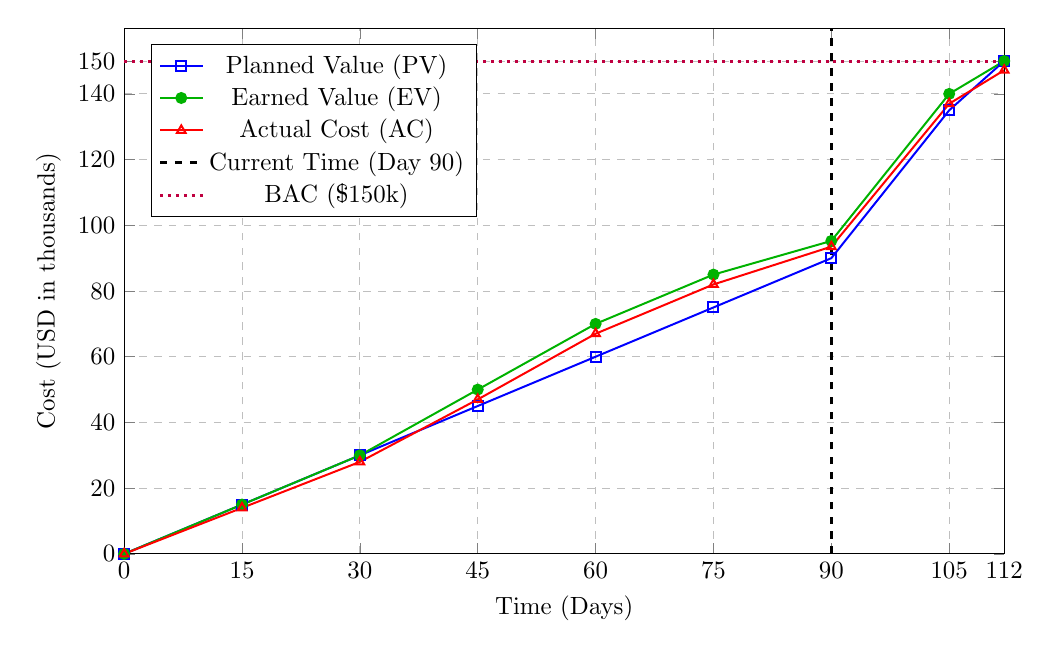
\begin{tikzpicture}[scale=0.9]
\begin{axis}[
    width=14cm,
    height=9cm,
    xlabel={Time (Days)},
    ylabel={Cost (USD in thousands)},
    xmin=0, xmax=112,
    ymin=0, ymax=160,
    xtick={0,15,30,45,60,75,90,105,112},
    ytick={0,20,40,60,80,100,120,140,150},
    legend pos=north west,
    ymajorgrids=true,
    xmajorgrids=true,
    grid style=dashed,
]

% Planned Value (PV) - Blue line
\addplot[
    color=blue,
    mark=square,
    thick,
    ]
    coordinates {
    (0,0)(15,15)(30,30)(45,45)(60,60)(75,75)(90,90)(105,135)(112,150)
    };
    \addlegendentry{Planned Value (PV)}

% Earned Value (EV) - Green line
\addplot[
    color=green!70!black,
    mark=*,
    thick,
    ]
    coordinates {
    (0,0)(15,15)(30,30)(45,50)(60,70)(75,85)(90,95.25)(105,140)(112,150)
    };
    \addlegendentry{Earned Value (EV)}

% Actual Cost (AC) - Red line
\addplot[
    color=red,
    mark=triangle,
    thick,
    ]
    coordinates {
    (0,0)(15,14)(30,28)(45,47)(60,67)(75,82)(90,93.5)(105,137)(112,147.2)
    };
    \addlegendentry{Actual Cost (AC)}

% Current time marker
\addplot[
    color=black,
    dashed,
    very thick,
    ]
    coordinates {
    (90,0)(90,160)
    };
    \addlegendentry{Current Time (Day 90)}

% BAC line
\addplot[
    color=purple,
    dotted,
    very thick,
    ]
    coordinates {
    (0,150)(112,150)
    };
    \addlegendentry{BAC (\$150k)}

\end{axis}
\end{tikzpicture}
\caption{Earned Value Management Chart showing PV, EV, and AC over project timeline}
\label{fig:ev_chart}
\end{figure}


\subsubsection{Chart Interpretation}

The Earned Value chart reveals several key insights:

\begin{enumerate}
    \item \textbf{Schedule Performance:} The EV line (green) is above the PV line (blue) at Day 90, confirming the project is ahead of schedule. The gap represents the \$5,250 schedule variance.
    
    \item \textbf{Cost Performance:} The EV line (green) is above the AC line (red), indicating the project is under budget. The vertical distance represents the \$1,750 cost variance.
    
    \item \textbf{Trend Analysis:} Both EV and AC curves show consistent upward trends that are favorable compared to the planned baseline. The project has maintained good performance throughout.
    
    \item \textbf{Future Projection:} Based on current trends (shown by the dotted projections), the project is expected to:
    \begin{itemize}
        \item Complete ahead of the planned 112-day schedule
        \item Finish under the \$150,000 BAC
        \item Maintain positive cost and schedule variances
    \end{itemize}
    
    \item \textbf{Risk Assessment:} The positive variances provide a buffer against potential risks in the remaining critical activities (Integration Testing, Deployment, and Closure phases).
\end{enumerate}

\subsection{Detailed Earned Value Management Analysis}

The following figures present the comprehensive Earned Value Management analysis including basic values, variance calculations, performance indices, forecasting, and detailed interpretation.

\begin{figure}[H]
\centering
\includegraphics[width=\textwidth,keepaspectratio]{earnedVal-1.png}
\caption{Earned Value Analysis - Basic values and assumptions}
\label{fig:ev1}
\end{figure}

\begin{figure}[H]
\centering
\includegraphics[width=\textwidth,keepaspectratio]{earnedVal-2.png}
\caption{Earned Value Analysis - Variance calculations and performance indices}
\label{fig:ev2}
\end{figure}

\begin{figure}[H]
\centering
\includegraphics[width=\textwidth,keepaspectratio]{earnedVal-3.png}
\caption{Earned Value Analysis - Forecasting and interpretation summary}
\label{fig:ev3}
\end{figure}

\newpage
\section{Conclusion}

This assignment has provided a comprehensive analysis of the Mindful Eating Agent project's scheduling, network dependencies, and cost management:

\subsection{Key Findings}

\textbf{Timeline and Scheduling:}
\begin{itemize}
    \item Total project duration: 112 days (September 1 - December 15, 2025)
    \item Critical path identified with 32 activities having zero slack
    \item AI/ML Module Development (24 days) and Mobile App Development (28 days) are the longest and most critical activities
    \item Clear assignment of responsibilities across three team members
\end{itemize}

\textbf{Network Analysis:}
\begin{itemize}
    \item AON network diagram clearly shows dependencies and parallel paths
    \item 8 non-critical activities provide scheduling flexibility
    \item UI/UX Design has the highest slack (8 days), providing design iteration flexibility
    \item Integration Testing (Day 86) is a critical merge point requiring careful monitoring
\end{itemize}

\textbf{Cost and Earned Value Management:}
\begin{itemize}
    \item Budget at Completion (BAC): \$150,000
    \item Current project status: Ahead of schedule (SPI = 1.058) and under budget (CPI = 1.019)
    \item Estimated completion cost: \$147,203 (saving \$2,797)
    \item Estimated completion time: 106 days (saving 6 days)
    \item Project health: Excellent, with positive variances in both cost and schedule
\end{itemize}


\subsection{Recommendations}

Based on the analysis, the following recommendations are made:

\begin{enumerate}
    \item \textbf{Maintain Focus on Critical Path:} Continue to closely monitor all critical path activities, especially AI/ML Module Development and Mobile App Development, as any delays will directly impact project completion.
    
    \item \textbf{Leverage Slack Time:} Utilize the slack time in non-critical activities (UI/UX Design, Database Design, Production Environment Setup) for quality improvements and additional testing.
    
    \item \textbf{Risk Mitigation:} Allocate additional resources to the Integration Testing phase (Day 86) as it is a critical merge point where delays could cascade.
    
    \item \textbf{Cost Management:} Continue current cost management practices as the project is performing well. The \$2,797 projected savings can be reallocated to quality assurance or user training.
    
    \item \textbf{Schedule Optimization:} Consider using the 6-day schedule buffer for extended user acceptance testing or early deployment preparation.
    
    \item \textbf{Continuous Monitoring:} Maintain regular EVM analysis to ensure the project continues on its positive trajectory and to identify any emerging issues early.
\end{enumerate}

\subsection{Final Remarks}

The Mindful Eating Agent project demonstrates strong project management practices with clear scheduling, well-defined dependencies, and effective cost control. The positive performance indicators suggest the project is well-positioned for successful completion within the planned timeframe and budget.

\end{document}
